\subsection{Running the system}

The system was fully deployed and ready to test: we were able to install the mobile application by downloading it directly from the Google Play Store; the webapp was hosted at \href{https://clup.cf}{https://clup.cf} (though it was not listed in the ITD document)

The backend REST API was also deployed and was available at \href{https://clup.cf/api/}{https://clup.cf/api/}

We also installed succesfully the mobile application using the provided build files.

\subsection{Building the backend}

Following the section 5 of the ITD, we installed the requirements Java JDK 15 (open-jdk) and Maven.

After pulling the repository from Github we run the command
\begin{lstlisting}
    $ mvn package -Dmaven.test.skip=true
\end{lstlisting}
on the folder IT/Implementation/Backend. The build was successful.
\begin{figure}[ht]
    \centering
    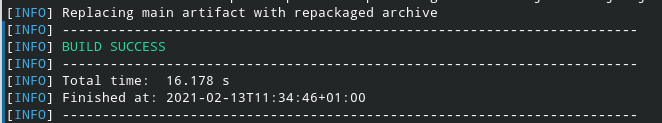
\includegraphics[width=\textwidth]{Images/package.jpg}
    \caption{\label{fig:Booked_Ticket_State}Result of the mvn package command.}
\end{figure}

\subsection{Deploying the backend locally}
As stated in the chapter 6 of the ITD a mysql data source should be available to the application, in order to make it work.

We hosted locally a mysql instance in a docker container and configured the application.yaml accordingly.


In the same folder of the application jar file we run
\begin{lstlisting}
    $ java -jar clupapplication-1.1.jar -spring.config.location=application.yaml
\end{lstlisting}

Connecting with a web browser at the address localhost:8084 (the port is configured in the application.yaml)
the CLup home page is displayed correctly. We tried to register an account, that worked properly.
\begin{figure}[ht]
    \centering
    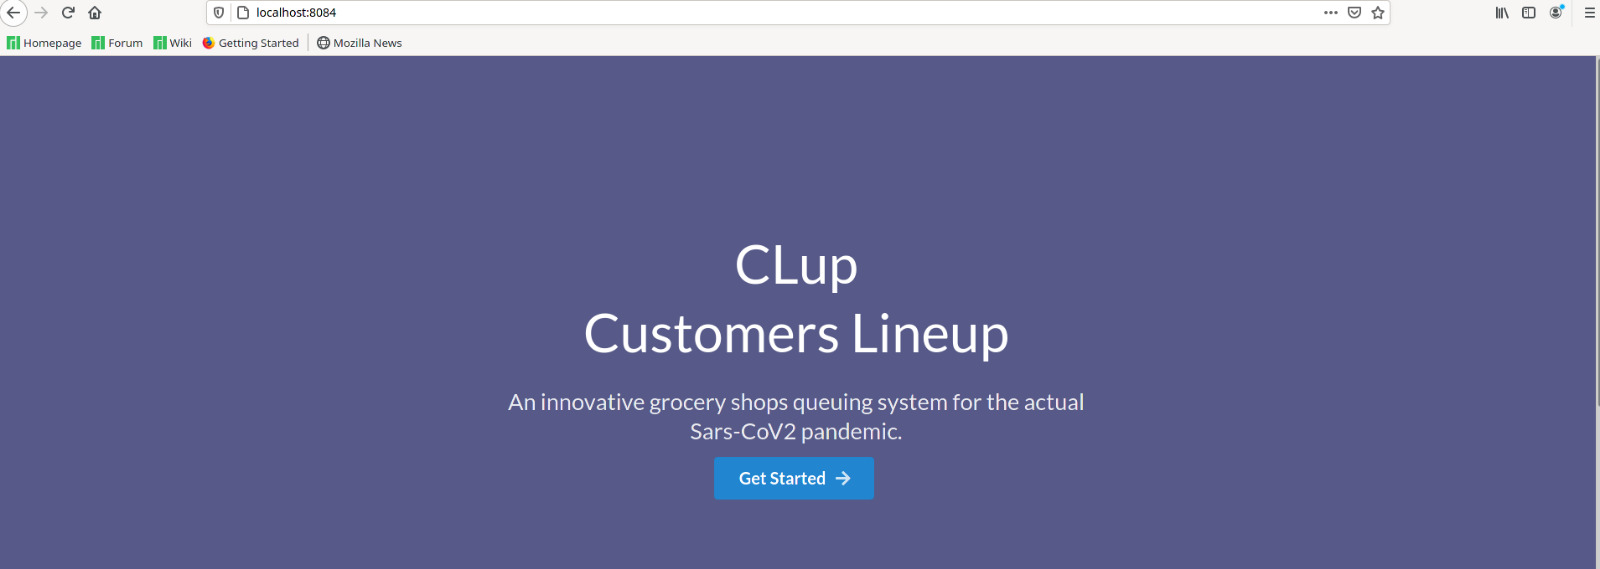
\includegraphics[width=\textwidth]{Images/deploy.jpg}
    \caption{\label{fig:Booked_Ticket_State}Homepage of the site deployed locally}
\end{figure}

\subsection{Running tests}
Using instruction in the chapter 5 we run the tests.
The application.yaml was not found in the folder specified by the instruction. Copying the application.yaml
file used in the deployment in the src/main/resources solves the issue (if the database used for testing is the
same used for the deployment).

After doing these steps running
\begin{lstlisting}
    $ mvn test
\end{lstlisting}
produces the following output
\begin{figure}[ht]
    \centering
    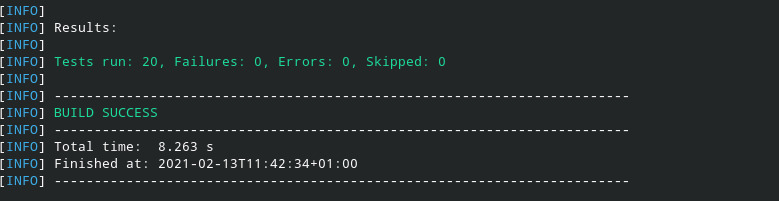
\includegraphics[width=\textwidth]{Images/test.jpg}
    \caption{\label{fig:Booked_Ticket_State}All tests passing}
\end{figure}
This means that all the test pass, as we expected.

%TODO: finish
% \subsection{Building from Source}

% Following the instructions to build the backend (using Java JDK 15) no issues were encountered,
